\documentclass[11pt, a4paper, oneside, parskip=full-]{scrartcl}

% -- PREABLE

% global settings
\renewcommand\labelitemi{-}

% packages
\usepackage[utf8]{inputenc}
\usepackage{graphicx} % to embed figures
\usepackage{float} % use [H] to place fig exactly where specified in code
\usepackage{tabularx} % table with columns that fill width of page using X
\usepackage{booktabs} % table utilities like \midrule
\usepackage{multirow} % span multiple rows in table
\usepackage{enumitem} % pass key-value config to itemize and enumberable
\usepackage{hyperref} % for links and urls
\usepackage[style=numeric,backend=biber,sorting=none]{biblatex} % For citing

\addbibresource{thesis.bib}

\graphicspath{ {img/} } % path where grahics are stored

% title page parameters
\title{Open-source GIS sandbox and data stories - A new tool for GIS workshops}
\author{Marc Folini}
\date{May 2022}

% -- BODY
\begin{document}

%-------------
% TITLE, ABSTRACT
%-------------
\begin{titlepage}
  \pagenumbering{Roman}
  \setcounter{page}{1}
  % create title page
  \clearpage\maketitle
  \thispagestyle{empty}
  % abstract
  \begin{abstract}
    It is desirable in GIS workshops to supplement the theoretical concepts with
    hands-on exercises in order for participants to become an active part in the
    learning experience. This requires that participants have access to an
    environment that provides the necessary software and data - ideally with
    minimal setup effort, independent of the system they use and easy to
    uninstall without leaving traces after the workshop. Different approaches
    were evaluated, and container technology was found to be a good fit to
    abstract away the hassle of setting up the tools and infrastructure. A proof
    of concept of what will be referred to as \emph{sandbox environment} was
    implemented and published as open source project.

    Furthermore, this thesis explored the concept of \emph{data stories}. A data
    story provides selected raw data, a motivating tangible goal and
    instructions that connect the raw data to the goal. It allows participants
    to fully focus on how the different tools interact with the data itself and
    other tools to achieve a meaningful result. This is in contrast to the
    majority of tutorials, which are tool focused and to which data is secondary
    to teach the necessary functionalities of a specific tool. An example data
    story was implemented whereby open data from the city of Zürich is used to
    derive a map showing what percentage of roads in each district are suitable
    for biking. Participants learn about GDAL's command line tools to inspect
    datasets and load them into PostGIS\cite{postgis}, where spatial processing
    and aggregation is performed. The result is made available as a new dataset
    to be consumed and styled in QGIS\cite{qgis}.
  \end{abstract}
\end{titlepage}

%-------------
% TABLE OF CONTENT
%-------------
\newpage
\tableofcontents

%-------------
% INTRODUCTION
%-------------
\newpage
\pagenumbering{arabic}
\setcounter{page}{1}
\section{Introduction}
Educational GIS\footnote{Geographic Information System (GIS).} workshops face a
few particular challenges, two of which are central to this thesis. Firstly, it
is generally desirable that participants can immediately experience theoretical
concepts hands-on for themselves. The challenge here lies in providing all
participants with access to the respective software and data with minimal setup
efforts. Secondly, the GIS landscape today consists of many components covering
the whole data lifecycle from initial data exploration to visualization and
distribution. Together with the myriad of commercial and open source tools for
each component, this might be overwhelming to unfamiliar participants.

This thesis was written as part of the CAS RIS 2021/22\footnote{Certificate of
advanced studies (CAS) in GIS (in German RIS) offered by ETH Zurich.}. It
explores the two above-mentioned challenges in the context of the CAS and aims
to address them on two different levels:
\begin{enumerate}
  \item \textbf{Infrastructure} In order to provide participants access to a
  variety of software with minimal setup effort the concept of a \emph{sandbox
  environment} is adopted. The requirements and components to be implemented in
  a first version were chosen to support the content of this thesis' further
  education curriculum.
  \item \textbf{Content} In order to help participants to make sense of the
  sandbox components and their interactions, the concept of a \emph{data story}
  was explored. Each data story has a tangible data use case goal statement that
  participants can identify with, for example: Let's visualize risk of wildfire
  and serve it as interactive map on a website. Starting from given raw data,
  participants follow the processing of this dataset through the different
  components and experience how they work together to achieve the goal.
\end{enumerate}


%-------------
% REQUIREMENTS
%-------------
\section{Requirements} \label{sectionrequirements} The content of the CAS RIS
was analyzed and assessed for potential hands-on exercises. From these findings
functional and non-functional requirements\footnote{Functional requirements
specify the tasks an application must be able to perform. Non-functional
requirements specify additional aspects about the application performing the
task, for example usability, look and feel or performance. } were then derived.

% Content analyis
%-------------
\subsection{Content analysis}
At the time of writing the course consisted of four weeks of content modules on
a wide variety of topics. Each module was screened with a focus on where
hands-on exercises could be added or expanded without substantially altering the
module structure or material. Modules focus primarily on usage of proprietary
software like ArcGIS were ignored. Table \ref{tab:tContentAnalysis} shows the
modules where hands-on potential was identified.

\begin{table}[!htbp]
  \centering
  \caption{Content analysis of existing lectures for hands-on potential.}
  \label{tab:tContentAnalysis}
  \begin{tabularx}{\textwidth}{lX}
    \toprule
    % header row start
    \textbf{Module} & \textbf{Hands-on potential} \\
    \midrule
    % row start
    Interoperabilität &
      \begin{itemize}[left=0pt,nosep,before={\begin{minipage}[t]{\hsize}},after
      ={\end{minipage}}]
      \item Inspection of and conversion between various data formats.
      \item Read Shapefile into a spatial database.
      \end{itemize}\nointerlineskip\\
    \midrule
    % row start
    SQL & Write and run basic SQL queries on sample data. \\
    \midrule
    % row start
    Geodatenbanken &
    \begin{itemize}[left=0pt,nosep,before={\begin{minipage}[t]{\hsize}},after
    ={\end{minipage}}]
      \item Run basic spatial queries on sample data.
      \item Perform spatial aggregation on sample data.
      \end{itemize}\nointerlineskip\\
    \midrule
    % multirow(4) start
    Geometrische Methoden & \multirow[t]{4}{*}{Run simple examples on sample
    data.} \\
    \cmidrule(r){1-1} Topologische Methoden &  \\
    \cmidrule(r){1-1} Mengenmethoden &  \\
    \cmidrule(r){1-1} Statistische Methoden &  \\
    \midrule
    % row start
    Einführung in Python & Self-study introduction of python basics. \\
    \midrule
    % row start
    Internet und GIS I \& II &
      \begin{itemize}[left=0pt,nosep,before={\begin{minipage}[t]{\hsize}},after
      ={\end{minipage}}]
      \item Load data from OGC web services WMS/WFS/WCS\footnote{The Open
      Geospatial Consortium (OGC) is a worldwide community to improve the access
      to geospatial data by various means such as developing standards. Such
      standards for the web include Web Map Service (WMS), Web Feature Service
      (WFS) and Web Coverage Service (WCS) to load styled map images, simple
      geometry features and raster data via http respectively.}.
      \item Optional: Consume WMS with QGIS. \end{itemize}\nointerlineskip \\
    \midrule
    % row start
    Projekt Internet \& GIS &
      \begin{itemize}[left=0pt,nosep,before={\begin{minipage}[t]{\hsize}},after
      ={\end{minipage}}]
      \item Use geodatabase as data source for OGC server.
      \item Create style and serve data as WMS.
      \item Consume WMS with QGIS. \end{itemize}\nointerlineskip \\
    \bottomrule
  \end{tabularx}%
\end{table}%

% Functional requirements
%-------------
\subsection{Functional requirements}
The following functional requirements were identified for the sandbox to be
useful in realizing the hands-on potential identified in the content analysis:
\begin{itemize}
  \item A spatial database is available together with utilities to import and
  query data.
  \item An OGC server implementation is available. There is a way to read
  predefined example data, read data from the user's system or connect to the
  sandbox spatial database.
  \item An OGC client implementation is available, which can interact with the
  sandbox OGC server or any other OGC service publicly available on the
  internet.
  \item The GDAL command line utilities, particularly gdalinfo and ogr2ogr, are
  available. There is a way to read either predefined example data or read data
  from the user's system.
  \item An environment to write and run python scripts which make use of the
  python geo-ecosystem. A use case would be to provide illustrative examples for
  the concepts of geometry, topology and spatial statistics.
\end{itemize}

% Non-Functional requirements
%-------------
\subsection{Non-Functional requirements}
\begin{itemize}
  \item Users can create content which is persisted between usages of the
  sandbox.
  \item There is a possibility to ship example scripts and data as part of the
  sandbox.
  \item Creation and distribution of data stories that are compatible with the
  tools of the sandbox should be possible without in-depth technological
  knowledge.
  \item The sandbox can be installed effortlessly and in a uniform way across
  the most common operating systems, namely Apple OS, Linux and Windows.
  \item The sandbox can be uninstalled without leaving traces on the operating
  system.
  \item Turning the sandbox on/off and accessing components should not require
  any programming knowledge.
  \item A partial or total reset of applications and data is possible in case
  something got messed up.
  \item Usage is not coupled to the duration of the CAS course or otherwise
  restricted (e.g. via externally controlled credentials).
\end{itemize}

%-------------
% SANDBOX
%-------------
\section{Sandbox}

% Existing projects
%-------------
\subsection{Existing projects}
The Google search engine was used to look for already existing similar projects
using various combinations of the terms \emph{gis}, \emph{geo}, \emph{sandbox},
\emph{workshop}, \emph{playground} and \emph{spatial}. No project was found that
satisfied the requirements outlined in section \ref{sectionrequirements}, but
some noteworthy findings are listed below.

\begin{itemize}
  \item Joeyklee's Geosandbox\cite{project-joeyklee} is a collection of
  tutorials which seems to focus on JavaScript client side mapping libraries
  such as Leaflet. It is not suitable for our purpose but mentioned here for the
  very similar name Geosandbox to avoid confusion.
  \item IDRE sandbox\cite{project-idre} does not provide any easy access to
  tools, but seems to be a collection of workshops and tutorials. It is
  mentioned here because the interesting goals and presentation of some
  workshops served as inspiration for the data story of this thesis.
  \item Digital Earth Australia (DEA) Sandbox\cite{project-dea} was a wonderful
  discovery. After creating a free account a cloud hosted JupyterJab platform
  with extensive python Juypter notebooks provide an interactive engaging
  experience to learn about the analysis of satellite imagery and much more. The
  DEA sandbox was a major inspiration for the heavy focus use of
  JupyterLab\cite{jupyterlab} in our sandbox.
  \item Geopython Workshop Repository\cite{project-geopython} is an extensive
  knowledge hub about a broad range of geospatial topics. The workshop is built
  on python Juypter notebooks using a containerized JupyterLab environment with
  pre-installed libraries. Docker compose is used as container orchestration
  technology. Even though the setup is too limited for the use case of this
  thesis (a spatial database is missing for example) the idea of using container
  technology to abstract away dependency management provided major inspiration
  for this thesis.
\end{itemize}

% Technology evaluation
%-------------
\subsection{Technology evaluation}

\subsubsection{High level architectural approaches}
The research on existing projects and further exploration of potential
technologies led to three distinct groups of architectural approaches. The
approaches are a) Sandbox as direct installation on user system, b) Sandbox as
local containerized application and c) Sandbox as cloud service.

\subsubsection*{Sandbox as direct installation on user system}
It was found that only four established open-source projects (QGIS, PostGIS,
pgAdmin\cite{pgadmin} and GeoServer\cite{geoserver}) would be enough to satisfy
the major part of the functional requirements. While the roles of PostGIS as
spatial database and GeoServer as OGC data server are well-defined, the QGIS
installation is particularly interesting because it comes bundled with versions
of GDAL\cite{gdal} and python that work together well and provides appropriate
interfaces. The community has produced installers for all major operating
systems, which makes the installation relatively straight-forward.

When it comes to non-functional requirements this approach falls short. A major
shortcoming is the lengthy and intrusive setup stemming from the lack of
separation of the sandbox software from the rest of the user's system. Depending
on already existing software and specific configurations this approach is at
best error-prone and at worst capable to permanently alter the user's system.
Because with this approach only the tools themselves are installed, tutorials
and data stories would need to be provided in a separate way. On the positive
side, the installed tools could be used beyond the duration of the CAS course
without problems and the decoupling of the distribution of tutorials and data
stories make it easy to be updated without technical knowledge.

\subsubsection*{Sandbox as local containerized application}
Container technology has been around for decades but took off in 2013 with the
release of Docker, which provided the tools that made container technology
accessible to the broader mass. Containers allow for bundling different software
components together in a reproducible way (an image) which can be distributed
and run in an isolated manner from the rest of the hosting computer's system
(called host). Compared to virtual machines containers are very lightweight and
can be started and stopped within seconds.

This approach takes the direct installation approach one step further by running
a spatial database or an OGC data server in containers isolated from the host
system. The environment within each container can be configured to be fully
tailored to the requirements. Complex installation procedures can be fully
abstracted away from the user as part of the image creation, which would allow
for example to set up a JupyterLab environment with system dependencies like
GDAL in order to have access to a wide variety of python packages from the
geo-ecosystem.

The setup complexity is comparatively low, because the only prerequisite is the
installation of Docker, which is an easy and mature process for all major
operating systems at this point thanks to its huge popularity. Once installed,
the containers can be started and stopped with single commands in seconds.
Containers can also contain data which optionally can be persisted on the host
on virtual volumes. Example scripts and data stories can be distributed as part
of the container and by using volumes they can be persisted across sandbox
restarts or selectively reset. Except for the initial installation this approach
satisfies all requirements.

\subsubsection*{Sandbox as cloud service}
The advances of container technology went hand in hand with the maturation of
the publicly available cloud. It's possible today even for a layman to run
containerized applications in the cloud at scale using a variety of managed
services ranging from authentication to load balancing.

This approach takes the local containerized approach one step further into the
cloud. Instead of bothering with the installation of Docker on the user's
computer and running the containers locally the sandbox is made available as a
service with a simple web interface and optionally some kind of login. Some
functional requirements such as the availability of a spatial database could
even be satisfied with cloud native components such as fully managed database
services.

The advantage of a cloud service is the low entry barrier because there is no
installation required. Example data and data stories can be made readily
available as part of the container setup and resetting is as simple as starting
a new sandbox cloud instance. This convenience comes at the price of a cost and
complexity overhead at the cloud side, because for persisting data across
sessions some form of authentication must be in place and every cloud session
uses resources which are billed by the second. Assuming the cloud sandbox is
publicly available to fulfill the requirement that the sandbox' usage should not
be coupled to the duration of the CAS course, further complexity arises from
implementing and maintaining security best practices against malicious attacks.
Data management is another topic which can prove challenging when it comes to
cloud services in the geospatial domain, because data usually needs to be
uploaded before being accessible and spatial data can quickly become rather
large for standard internet connection upload speeds leading to disruptions and
waiting times.

\subsubsection*{Conclusion}
All three approaches satisfy the functional requirements, which is why the
non-functional requirements will be used to argue for the final decision. The
direct installation approach falls short here. The local containerization
approach has some minor shortcomings when it comes to the initial installation,
but shines in almost all other areas. The cloud service approach is the
opposite, shining with a zero-effort setup but falling behind the local
containerization approach in terms of maintainability, cost, and data
management.

The approach \emph{Sandbox as local containerized application} was eventually
chosen for the further implementation, because simplicity of a local setup
combined with the advantages of container technologies was found to outweigh the
cost of the initial setup, which is still orders of magnitude simpler than with
the direct installation approach.

\subsubsection{Technology evaluation for local containerized setup}
The technology to be used for local containerized setup has to be able to run
multiple containers which can communicate among each other as well as with the
host system and store data which is persisted beyond the lifecycle of each
container. Among many possibilities, three technologies were considered more
closely due to their popularity and the availability of detailed documentation:
Docker Compose, Docker Swarm and Minikube.

\begin{itemize}
  \item \textbf{Docker Compose}\cite{dockercompose} is a tool that allows to run
  multi-container applications on a single host. A single compose file acts as
  configuration for container lifecycle and environment as well as the
  networking and storage layers.
  \item \textbf{Docker Swarm}\cite{dockerswarm} shares many concepts with Docker
  Compose and can be considered an evolution towards orchestrating multiple
  containers across multiple host machines. It is also possible to run Docker
  Swarm on a single host machine.
  \item \textbf{Minikube}\cite{minikube} is a tool that lets you run a local
  version of a Kubernetes Cluster. Kubernetes is one of the most popular
  container orchestration softwares and at a high level similar to Docker Swarm.
  It provides its own approach towards managing containers, networking and
  storage which is generally more targeted towards large-scale enteprise
  applications.
\end{itemize}

All three technologies were evaluated on a two container setup of a spatial
database (PostGIS) and an associated administrator application (pgAdmin). While
all three technologies provided extensive documentation that allowed for
successful testing, Docker Compose proved to be the simplest solution in terms
of inital setup and ease of use, due to its single configuration file and the
targeted usecase to run on a single host. To that end \emph{Docker Compose} was
chosen as the technology to implement the \emph{Sandbox as local containerized
application}.


% Docker Compose architecture
%-------------
\subsection{Docker Compose architecture}

At the heart of a Docker Compose application is a configuration file, called
\emph{compose file} which describes the components of the multi-container
application and how they interact. Each component is called a \emph{service},
which consists of an image that specifies the containerized application at the
heart of the service and additional configuration about how to interact with
other services or how to be accessible from the host system. When the Docker
Compose application is startet, the images of each service are used to start
containers within which the application of interest then runs. A compose file
can also declare \emph{volumes}, which can be used by services to save data
which should be persisted across restarts of a service.

The architecture of the sandbox is outlined in Figure \ref{fig:sandboxsetup}.
The following containerized applications are provided as downloadable images by
third parties and used without modifications:

\begin{itemize}
  \item \textbf{postgis-container}\cite{postgis-container} is a containerized
  version of PostGIS, a spatial database. The container uses a volume called
  postgis-data to persist the database content.
  \item \textbf{pgadmin-container}\cite{pgadmin-container} is a containerized
  version of pgAdmin4, a graphical user interface to facilitate the
  administration of PostgreSQL based databases, such as PostGIS. The container
  uses a volume called pgadmin-data to persist configurations, such as database
  connections.
  \item \textbf{geoserver-container}\cite{geoserver-container} is a
  containerized version of Geoserver, which is an OGC data server and a
  reference implementation of the OGC web standards . The version used priovided
  by Kartoza and has configuration options to include community extensions,
  plugins and sample data. The container uses a volume called geoserver-data to
  persist its configuration and data directories.
\end{itemize}

The following components were created in the course of this thesis and the code
is provided in this thesis' repository\cite{osgeostacksandbox}:

\begin{itemize}
  \item \textbf{geoscriptingsandbox-container} is a containerized version of
  JupyterLab with various preinstalled python packages from the geo-ecosystem
  and fundamental libraries such as GDAL and GEOS\cite{geos}. This setup allows
  users to explore the python geo-ecosystem as well as the various command line
  utilities that GDAL offers. The expressive nature of Jupyter Notebooks is also
  used to visualize the data stories. The container uses a volume called
  geoscriptingsandbox-data to persist user created Jupyter notebooks and data.
  \item \textbf{datastories-container} is called a data container because it
  serves solely as a data storage without application. It contains the data
  story related narrative in form of Jupyter notebooks as well as the sample
  data. Upon start, it copies all its content to a volume datastories-data which
  can be accessed by other components such as geoscriptingsandbox-container to
  run through the data story notebooks.
  \item \textbf{hub-container} runs a simple web application that serves as an
  entry point and central. Here a user finds links to access other sandbox
  components and the relevant connection information. The hub is the first thing
  a user sees when typing \emph{localhost} in the browser after starting the
  sandbox.
\end{itemize}

\begin{figure}[H]
  \centering
  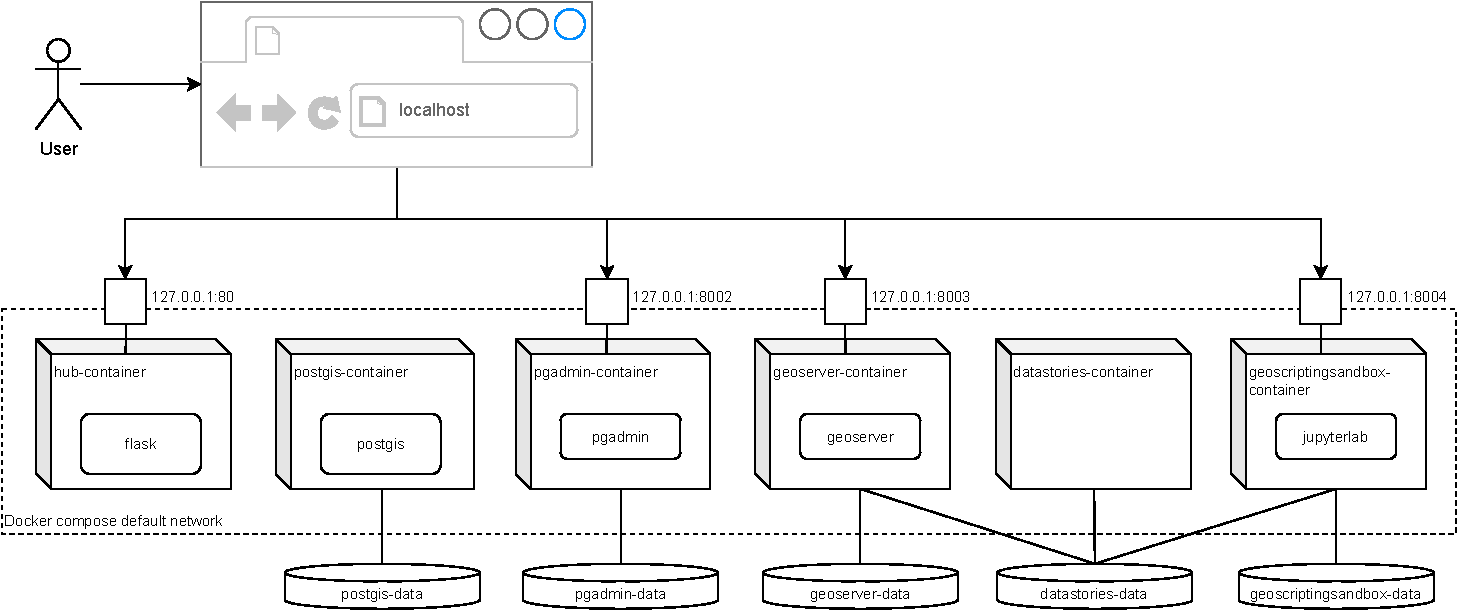
\includegraphics[width=1\textwidth]{composeSetup}
  \caption{Sandbox setup using docker compose}
  \label{fig:sandboxsetup}
\end{figure}


% Using the sandbox
%-------------
\subsection{Sandbox setup and usage}


%-------------
% DATA STORY
%-------------
\section{Data story}


%-------------
% CONCLUSION
%-------------
\section{Conclusion}


%-------------
% REFERENCES
%-------------
\printbibliography

\end{document}
